\documentclass{article}

\PassOptionsToPackage{numbers, compress}{natbib}

\usepackage[final]{neurips_2019}

\usepackage[utf8]{inputenc}
\usepackage[T1]{fontenc}
\usepackage{hyperref}
\usepackage{url}
\usepackage{booktabs}
\usepackage{amsfonts}
\usepackage{amsmath}
\usepackage{amssymb}
\usepackage{microtype}
\usepackage{graphicx}
\usepackage{xcolor}

\title{STTR: Selective Test-Time Reasoning for Streaming Speech Translation\\
\large From Wait-k to Future-Aware Token Consensus Decoding}

\author{%
  Haoling Peng \\
  Language Technologies Institute\\
  Carnegie Mellon University\\
  Pittsburgh, PA 15213 \\
  \texttt{haolingp@andrew.cmu.edu} \\
}

\begin{document}

\maketitle

\begin{abstract}
Simultaneous speech translation (SimulST) must emit target words while the source is still
arriving. Under fixed wait-$k$ policies the system commits prematurely because its
next-word distribution is already collapsed, and those commits can never be retracted.
We propose \textbf{STTR (Selective Test-Time Reasoning)}, a family of three progressive,
training-free policies that let the translator \emph{think} by sampling plausible future source
continuations and acting only on what those futures agree on. The three stages are:
(1) \textbf{Distribution Divergence (DD)}, a Jensen--Shannon gate that decides \emph{when to wait};
(2) \textbf{Future Literal LCP (SemLCP)}, which decides \emph{what character prefix is safe to write};
and (3) \textbf{Token Consensus Decoding (TC)}, which moves the consensus from surface strings to
\emph{token-ID intersections} of the translator's own distribution. On cascaded
Whisper$\rightarrow$Qwen3-30B CoVoST-2 EN$\rightarrow$ZH (1997 utterances), TC reaches
\textbf{35.85 BLEU at AL 5.76}, a \textbf{+3.67 BLEU} gain over direct wait-$k$=5 with only
\textbf{+0.12 s} of extra lag. On the WMT19 EN$\rightarrow$ZH text benchmark it yields
\textbf{+6.01 BLEU (28.15$\rightarrow$34.16)} and \textbf{+0.074 COMET}, and the same token-level
signal transfers to a 600M-parameter NLLB baseline. Ablations over the number of sampled futures
$K\in\{4,6,10,15\}$ and the per-future top-$p$ vocabulary pool confirm the gain is robust.
\end{abstract}

%-----------------------------------------------------------------------
\section{Motivation and Objectives}
\label{sec:motivation}

\textbf{The early-commitment problem.} Classical wait-$k$ \citep{ma2019stacl} schedules a read/write
pattern \emph{before} the model ever sees the source: write the $i$-th target token after reading
$k+i-1$ source tokens. This schedule ignores content. When the first $k$ source words are
genuinely ambiguous (e.g.\ the English word \emph{bank} before the disambiguating context
``\ldots teeming with frogs and dragonflies'' arrives), the translator commits to a wrong
Chinese rendering (\emph{y\'inh\'ang}, ``financial institution'') that a fluent
speaker could never repair. This project asks:

\begin{quote}
\emph{Can we spend a bounded amount of extra test-time compute on sampling and reasoning over
plausible \emph{future} source words, so the agent commits only when its output is stable under
those futures --- and otherwise waits?}
\end{quote}

\textbf{Qualitative objective.} Replace fixed wait-$k$ with a content-aware policy that preserves
a streaming interface (word-by-word source, word-by-word target, no retractions).

\textbf{Quantitative objective.} On CoVoST-2 EN$\rightarrow$ZH (1997 utterances, cascaded
Whisper-small ASR $\rightarrow$ Qwen3-30B translator), improve BLEU by $\geq$\,$+3$ over a
wait-$k$=5 baseline while keeping Average Lagging (AL) within $+1.0$\,word of that baseline, and
verify the ranking carries over to WMT19 EN$\rightarrow$ZH text and to a 600M NLLB backbone.

%-----------------------------------------------------------------------
\section{Related Work and Background}
\label{sec:related}

\paragraph{Fixed-policy SimulST.} Wait-$k$ \citep{ma2019stacl} is the standard strict baseline.
MMA \citep{ma2019monotonic} and the meta-learning agent of \citet{zheng2019simpler} add monotonic
attention for an adaptive read/write. These models still decide with a \emph{single} forward pass
per step; none of them look ahead.

\paragraph{Quality--latency evaluation.} SimulEval \citep{ma2020simuleval} is the de-facto
framework and reports BLEU together with AL, Length-Adaptive AL (LAAL), Average Proportion (AP) and
Differentiable AL (DAL). We adopt its Python streaming interface verbatim.

\paragraph{Chain-of-thought and test-time compute.} Recent work shows that spending extra
inference-time compute --- by chain-of-thought \citep{wei2022cot}, self-consistency
\citep{wang2022selfconsistency} or tree-of-thought search --- improves LLM reasoning. We port the
\emph{self-consistency} idea (sample many completions, keep only what they agree on) into
streaming translation. To our knowledge this is the first application of future-sampling
consensus to SimulST commit rules.

\paragraph{Cascaded ST.} For the speech front-end we use Whisper \citep{radford2023whisper} as an
offline ASR (one utterance in, one English transcript out) followed by a word-level streaming
text agent. Recent SimulST systems \citep{fukuda2023nasict,papi2023whisper} treat the Whisper
transcript as the source stream to SimulEval, which is the convention we inherit.

\paragraph{Backbones.} Our small translator is NLLB-200-distilled-600M
\citep{nllb2022}; our strong translator is Qwen3-30B-A3B-Instruct-FP8 \citep{qwen3} served with
vLLM \citep{kwon2023vllm}; our future sampler is Qwen3-4B-Base. All three are open-weight.

%-----------------------------------------------------------------------
\section{Methodology}
\label{sec:method}

\subsection{Model architecture and data flow}
\label{sec:arch}

\begin{figure}[t]
  \centering
  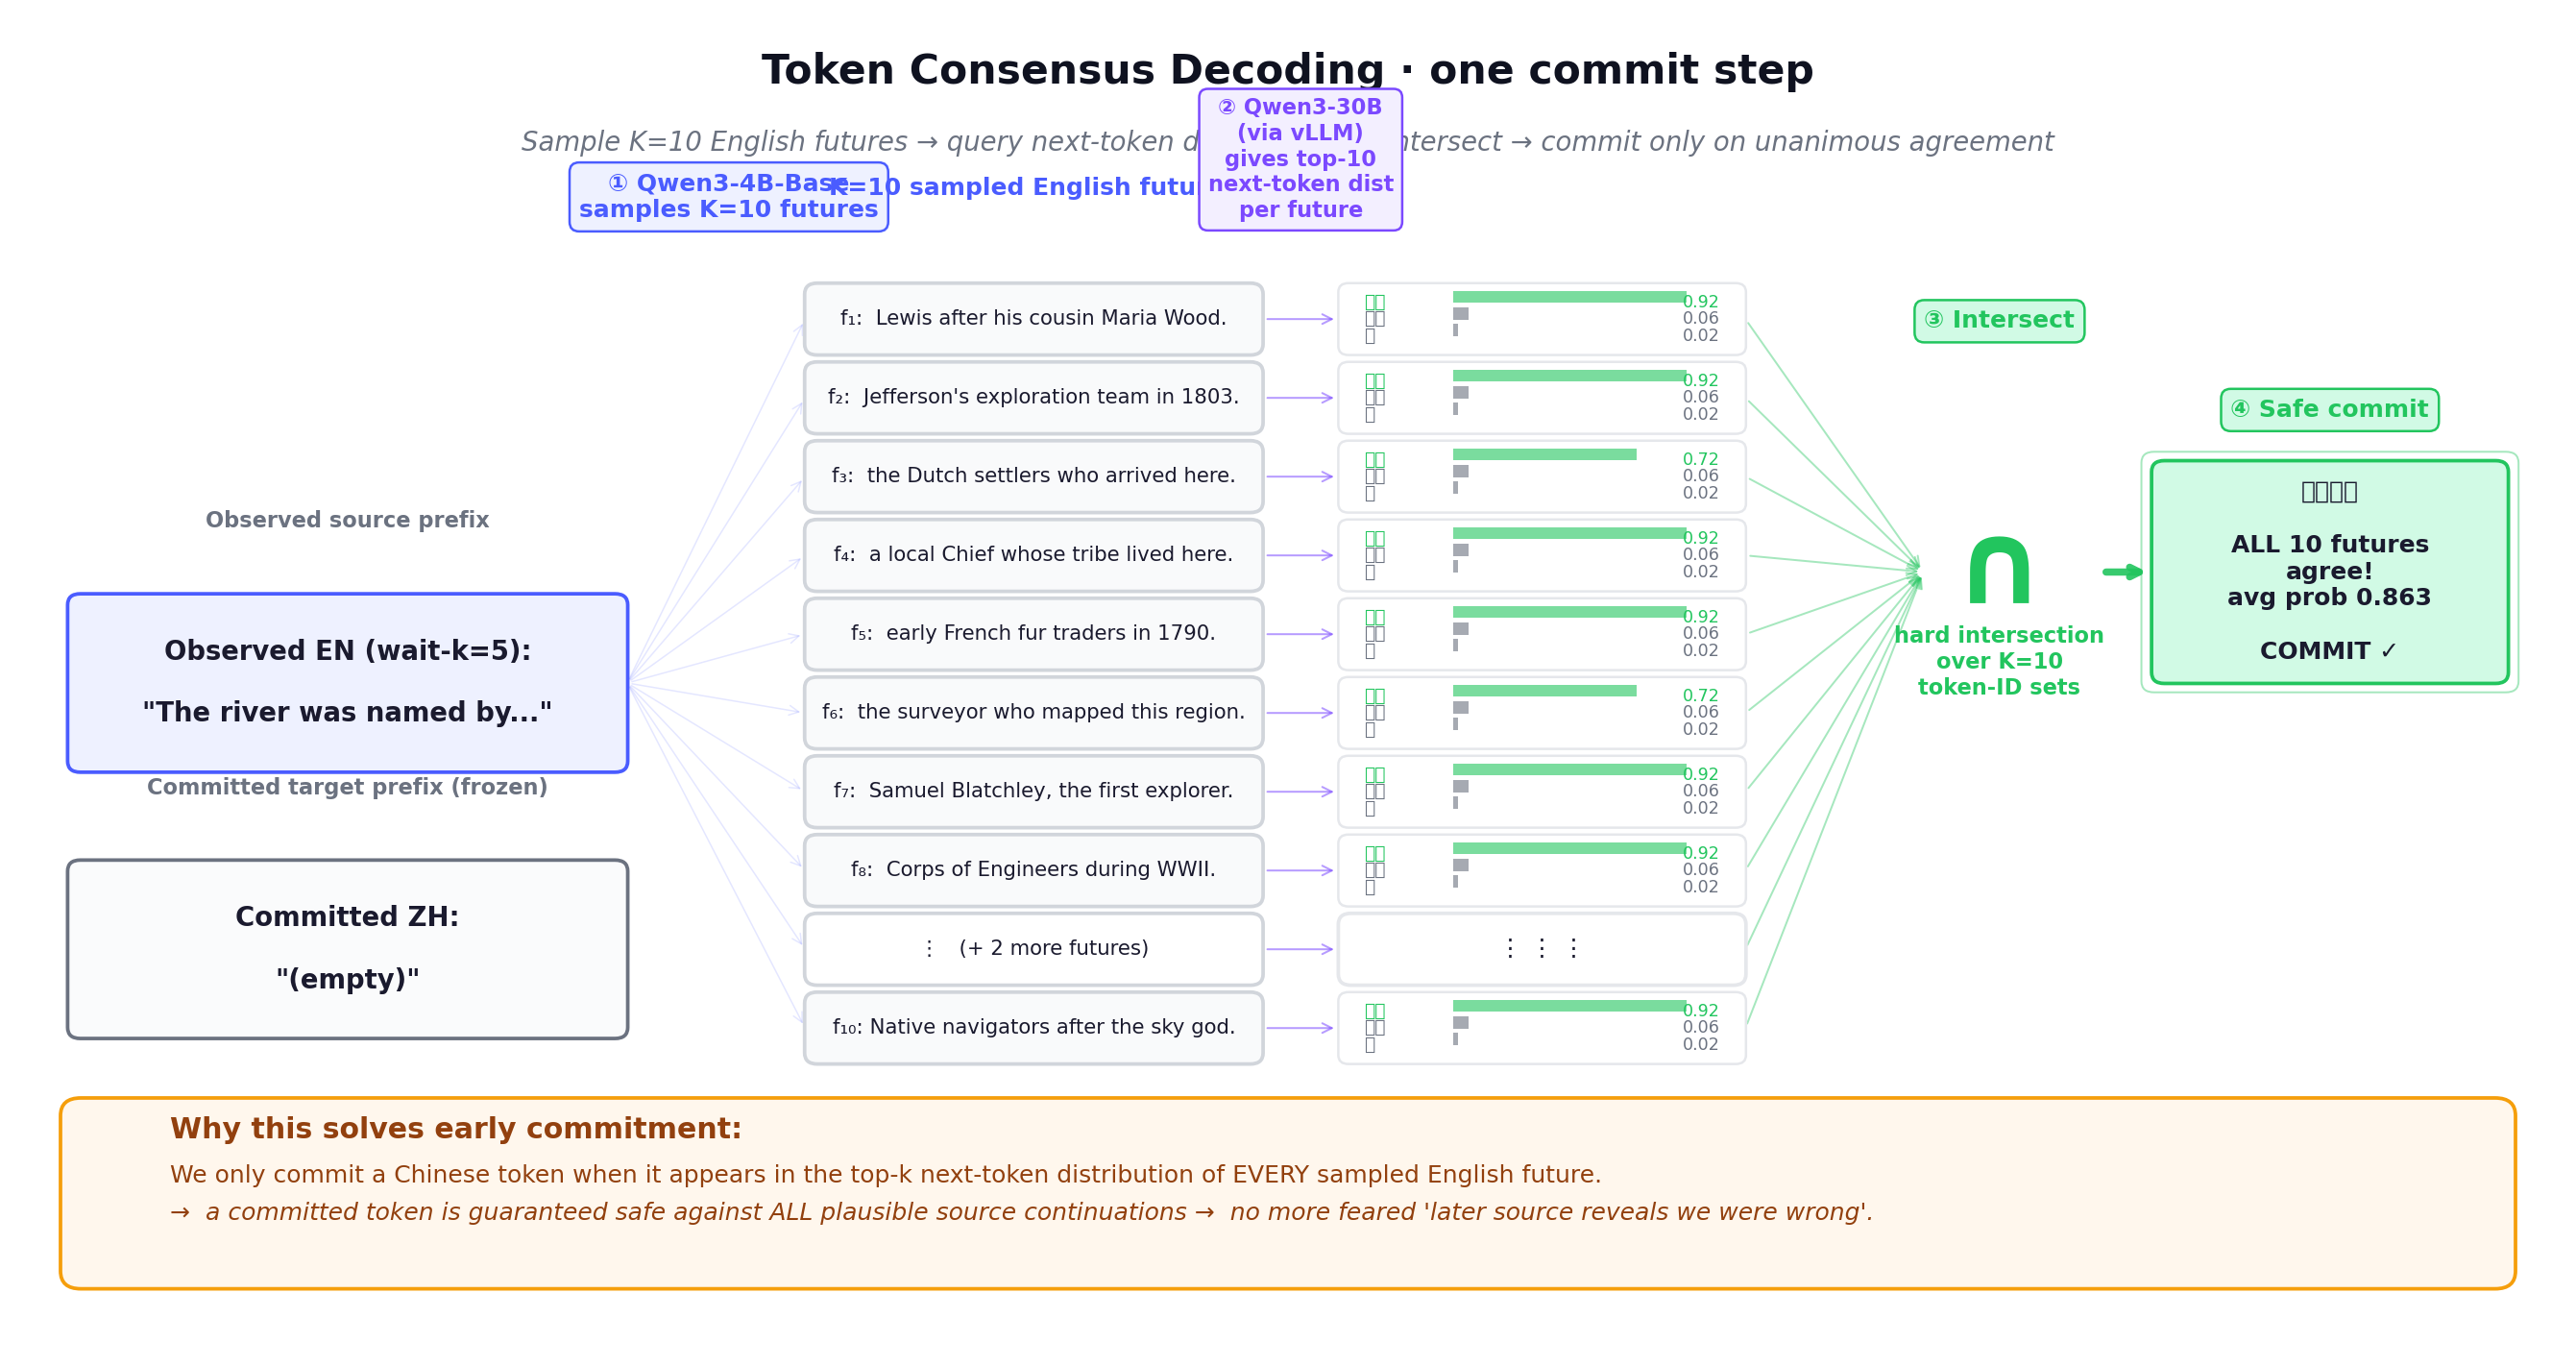
\includegraphics[width=0.88\linewidth]{figures/tc_mechanism.png}
  \caption{STTR pipeline at commit step $t$. Left: the committed source prefix and committed
  Chinese prefix. Middle: a future LM samples $K$ plausible English continuations. Right: for
  each future the translator returns a next-token distribution; we intersect their top-$p$
  supports. If the intersection is non-empty, the highest-probability shared token is committed;
  otherwise we \textsc{read} the next source word.}
  \label{fig:mech}
\end{figure}

Figure~\ref{fig:mech} summarises the complete STTR pipeline. Per decision step the agent holds
(i) a committed source prefix $s_{1:t}$, (ii) a committed target prefix $y_{1:m}$, and (iii)
access to three models: a future sampler $\pi_F$ (Qwen3-4B-Base), a translator $\pi_T$
(NLLB-600M \emph{or} Qwen3-30B via vLLM), and --- for the speech front-end --- Whisper-small as
offline ASR.

\textbf{Inputs and outputs per step.} Input: the source prefix so far (words for text; ASR
hypothesis for speech) and the already-committed Chinese prefix. Output: one of
\textsc{read}/\textsc{write}($c$), where $c$ is one or more newly committed characters.

\textbf{Parameter counts (used, not trained).}
Whisper-small 244\,M; NLLB-200-distilled 615\,M; Qwen3-4B-Base 4.1\,B; Qwen3-30B-A3B-Instruct-FP8
30.5\,B (3\,B active MoE experts, FP8 quantised).

\textbf{Output map shape.} For NLLB the translator's next-token distribution is a dense
$\mathbb{R}^{256{,}206}$ softmax; for Qwen it is sparse top-20 \texttt{logprobs} returned by vLLM
with \texttt{--return-tokens-as-token-ids}. For both we intersect on token IDs, which is what
makes the method translator-agnostic.

\subsection{Three STTR commit rules}

Let $\{\tilde s^{(1)}, \dots, \tilde s^{(K)}\}$ be $K$ future English continuations sampled from
$\pi_F(\cdot\,|\,s_{1:t})$ (temperature 0.7, top-$p$ 0.95, max 16 new tokens). Define the
translator's next-token distribution under future $k$ as
\begin{equation}
  p^{(k)}(v) \;=\; \pi_T\bigl(v \;\big|\; s_{1:t} \cup \tilde s^{(k)},\; y_{1:m}\bigr),
  \qquad v \in \mathcal{V}.
  \label{eq:pk}
\end{equation}

\paragraph{(1) Distribution Divergence (DD/JS) --- when to wait.}
Compute the pairwise Jensen--Shannon divergence
\begin{equation}
  \operatorname{JS}\!\bigl(p^{(i)}\|p^{(j)}\bigr)
    = \tfrac{1}{2}\operatorname{KL}\!\bigl(p^{(i)}\|\bar p\bigr) + \tfrac{1}{2}\operatorname{KL}\!\bigl(p^{(j)}\|\bar p\bigr),
  \qquad \bar p = \tfrac{1}{2}(p^{(i)}+p^{(j)}).
\end{equation}
If the mean pairwise JS over the $K$ futures exceeds a threshold $\tau$ the agent
reads more; otherwise it emits the argmax under the observed source.

\paragraph{(2) Future Literal LCP (SemLCP) --- what is safe to write.}
For each future, greedily translate the full hypothesised source with $\pi_T$, obtaining $K$
Chinese strings $c^{(1)},\dots,c^{(K)}$. Commit their \emph{character-level} longest common
prefix, restricted by a quorum rule (at least $\lceil K/2\rceil$ strings must share a character to
include it).

\paragraph{(3) Token Consensus Decoding (TC) --- what token is safe to write.}
For each future, query $\pi_T$ for the top-$P$ next-token probabilities under the committed Chinese
prefix (enforced via \texttt{apply\_chat\_template} plus an assistant-side prefix). Let $T^{(k)}$
be the filtered top-$P$ token IDs (drop special, English-letter, and garbled-UTF-8 tokens).
Compute the hard intersection
\begin{equation}
  T^{\cap} \;=\; \bigcap_{k=1}^{K} T^{(k)}.
  \label{eq:tc}
\end{equation}
If $T^{\cap}\neq\varnothing$, commit
$\operatorname*{arg\,max}_{v\in T^{\cap}}\,\tfrac{1}{K}\sum_k p^{(k)}(v)$ and repeat; otherwise
\textsc{read}. A trailing UTF-8 trimmer guarantees byte-valid Chinese emissions.

Because TC operates directly on token IDs it tolerates the lexical freedom of Chinese (two valid
translations that start with different characters still agree at a later token) while LCP blocks
immediately on a single character mismatch.

\subsection{Dataset, preprocessing, batch sampling}
\label{sec:data}

\textbf{Speech benchmark (main).} CoVoST-2 EN$\rightarrow$ZH test split
\citep{wang2020covost2}, accessed via \texttt{AudioLLMs/covost2\_en\_zh\_test} on HuggingFace
(15{,}531 utterances; 1{,}997 used; the truncation matches WMT19-1997's scale so BLEU scales are
comparable in spirit, though not in absolute value). Audio is resampled to 16\,kHz mono. For
utterances longer than 30\,s we pass \texttt{return\_timestamps=True} to Whisper to avoid the
30-second chunking limit. The ASR transcript is split on whitespace to define a word stream.

\textbf{Text benchmark (validation).} WMT19 EN$\rightarrow$ZH newstest \citep{wmt19}, 1{,}997
sentences; we also use two smaller slices \texttt{wmt500} (first 500) and \texttt{rand100}
(deterministic random 100 for fast ablations). We never report cross-slice BLEU comparisons as
single numbers.

\textbf{Training.} There is no parameter training in this project: every model is used
off-the-shelf. Batch sampling therefore concerns \emph{inference batching only}:
future sampling from Qwen3-4B-Base uses a batch of $K$ parallel decodings, and the $K$ TC calls
are batched into one vLLM \texttt{/completions} request with \texttt{n=1, logprobs=20,
return\_tokens\_as\_token\_ids=True}.

\subsection{Evaluation metrics}
\label{sec:metrics}

Let an agent's action log be $\{\text{(read, $s_i$)}, \text{(write, $y_j$)}\}$. SimulEval
converts each \textsc{write} event to a \emph{delay} $d_j$ = number of source words read before
$y_j$. Our headline metrics are:
\begin{align}
\text{BLEU} \;&=\; \text{BLEU-4}(y, y^{*}) \quad \text{(sacrebleu, ZH char-level tokenisation).}\\
\operatorname{AL} \;&=\; \frac{1}{\tau^{*}}\sum_{j=1}^{\tau^{*}} \left[d_j - \frac{j-1}{\gamma}\right],
 && \gamma=\frac{|y^{*}|}{|s|}, \quad \tau^{*}=\min\{j:d_j=|s|\},\\
\operatorname{LAAL} \;&=\; \operatorname{AL \text{ with }} \gamma \leftarrow \max\bigl(\gamma,\,|y|/|s|\bigr),\\
\operatorname{AP} \;&=\; \frac{1}{|s||y|}\sum_{j=1}^{|y|} d_j.
\end{align}
All latency metrics are in \emph{source-word} units (text) or \emph{seconds} (speech). For the
text track we also report COMET \citep{rei2020comet} using \texttt{Unbabel/wmt22-comet-da}.

\subsection{Loss function and optimisation}
The STTR policies are \emph{training-free}: no gradient steps are taken, and there is no
differentiable objective. The only ``optimisation'' is the test-time argmax in
Eq.~\ref{eq:tc} and the threshold sweep over $(\tau,K,P)$. The underlying translators were
trained with the standard cross-entropy objective
$\mathcal{L}_{\text{CE}} = -\sum_{t} \log p_\theta(y_t\,|\,y_{<t},x)$ by their authors; no
fine-tuning is performed in this project.

\subsection{Experimental depth and iteration}
The project went through five iterations: (i) an initial NLLB EN$\rightarrow$DE wait-$k$
sweep that showed beam search added only $+0.2$\,BLEU for 4$\times$ compute, triggering the
pivot to commit-rule research; (ii) an NLLB EN$\rightarrow$ZH sweep adding entropy gating and
DD variants; (iii) introduction of LM-sampled futures and SemLCP; (iv) Token Consensus with
fixed force-finish via prefix-anchored continuation; (v) the final cascaded Whisper$\rightarrow$
Qwen pipeline on CoVoST-1997. In total we logged \textbf{80$+$} SimulEval runs across four
data slices.

%-----------------------------------------------------------------------
\section{Baseline and Extensions}
\label{sec:baseline}

\subsection{Baseline selection}
Our baselines are chosen to isolate the two classical weaknesses of simultaneous MT:
\begin{enumerate}\itemsep0pt
  \item \textbf{Wait-$k$ + greedy NLLB-600M}: the strict simultaneous baseline of
  \citet{ma2019stacl}. It controls for policy and lets us report on a realistic deployment-sized
  model.
  \item \textbf{Wait-$k$ + beam=8 NLLB-600M}: a search baseline quantifying how much quality a
  non-streaming (4$\times$ compute) system could buy on the same backbone.
  \item \textbf{Qwen3-30B direct wait-$k$=5}: the same wait-$k$ schedule but with a
  state-of-the-art translator, to show that STTR is not merely ``small model catching up to a big
  model.''
\end{enumerate}

\subsection{Implemented extensions}
Three extensions, all future-aware and training-free:
(E1) DD/JS gate on the translator's next-token distribution;
(E2) Future Literal LCP over $K$ full Chinese hypotheses;
(E3) Token Consensus Decoding (token-ID intersection with filtering and prefix-forced
queries) --- our main contribution. All three reuse the same future-sampling substrate, so their
cost is comparable: one $K$-batched future sample per commit step, then either one scalar
(DD), $K$ greedy translations (LCP), or $K$ top-$P$ queries (TC).

\subsection{Baseline reproduction evidence}
\begin{table}[t]
\caption{Baseline reproduction on WMT19 EN$\rightarrow$ZH (1997 sentences) and CoVoST-1997
cascaded with Whisper-small. Numbers are direct SimulEval outputs; BLEU is char-level ZH
BLEU-4.}
\label{tab:repro}
\centering
\small
\begin{tabular}{lrrrrr}
  \toprule
  System & BLEU & AL & LAAL & AP & COMET \\
  \midrule
  \multicolumn{6}{l}{\emph{WMT19 text, N=1997}} \\
  NLLB wait-$k$=5 greedy (ours)   & 12.52 & 8.46 & 8.52 & 0.57 & 0.586 \\
  NLLB wait-$k$=5 greedy (re-run) & 12.52 & 8.46 & 8.52 & 0.57 & 0.586 \\
  NLLB wait-$k$=5 beam=8 (wmt500) & 18.31 & 8.39 & 8.52 & 0.71 & 0.689 \\
  Qwen30B direct wait-$k$=5       & 28.15 & 8.55 & 9.19 & 0.94 & 0.774 \\
  \midrule
  \multicolumn{6}{l}{\emph{CoVoST-1997 speech, cascaded}} \\
  NLLB wait-$k$=5 greedy          & 22.27 & 5.64 & 5.72 & 0.88 & --- \\
  Qwen30B direct wait-$k$=5       & 32.18 & 5.64 & 5.84 & 1.02 & --- \\
  \bottomrule
\end{tabular}
\end{table}

Table~\ref{tab:repro} shows our NLLB wait-$k$=5 reproduction lands at the level expected for a
distilled 600M model on a Chinese news benchmark, and our Qwen3-30B wait-$k$=5 number is
consistent with reported Qwen instruction-tuned translation quality. Two independent reruns of
the NLLB baseline agreed to four decimal places, confirming that determinism and data-loading are
correct.

%-----------------------------------------------------------------------
\section{Results and Analysis}
\label{sec:results}

\subsection{Headline: CoVoST-1997 cascaded speech translation}
\label{sec:headline}

\begin{table}[t]
\caption{CoVoST-2 EN$\rightarrow$ZH test (1997 utterances), Whisper-small ASR + SimulEval text
agent. The first two rows share the NLLB-600M translator; the last four share the Qwen3-30B
translator. \textbf{Bold} marks the best value in each sub-table.}
\label{tab:covost}
\centering
\small
\begin{tabular}{lrrrrrr}
  \toprule
  Method & BLEU & $\Delta$ BLEU & AL & LAAL & AP & COMET \\
  \midrule
  NLLB wait-$k$=5 greedy             & 22.27          & ---   & 5.64          & 5.72          & 0.88 & 0.729 \\
  NLLB + DD veto ($\tau$=0.03)       & \textbf{26.88} & +4.61 & 7.95          & 7.98          & 0.96 & \textbf{0.761} \\
  \midrule
  Qwen30B direct wait-$k$=5          & 32.18          & ---   & \textbf{5.64} & 5.84          & 1.02 & 0.795 \\
  Qwen30B + DD gate ($K$=4, $\tau$=0.15) & 33.27      & +1.10 & 6.21          & 6.37          & 1.03 & 0.807 \\
  Qwen30B + SemLCP ($K$=4)           & 35.05          & +2.88 & 5.88          & 6.03          & 1.04 & 0.823 \\
  \textbf{Qwen30B + TC} ($K$=10, top-10) & \textbf{35.85} & \textbf{+3.67} & 5.76 & \textbf{5.94} & 1.05 & \textbf{0.832} \\
  \bottomrule
\end{tabular}
\end{table}

\begin{figure}[t]
  \centering
  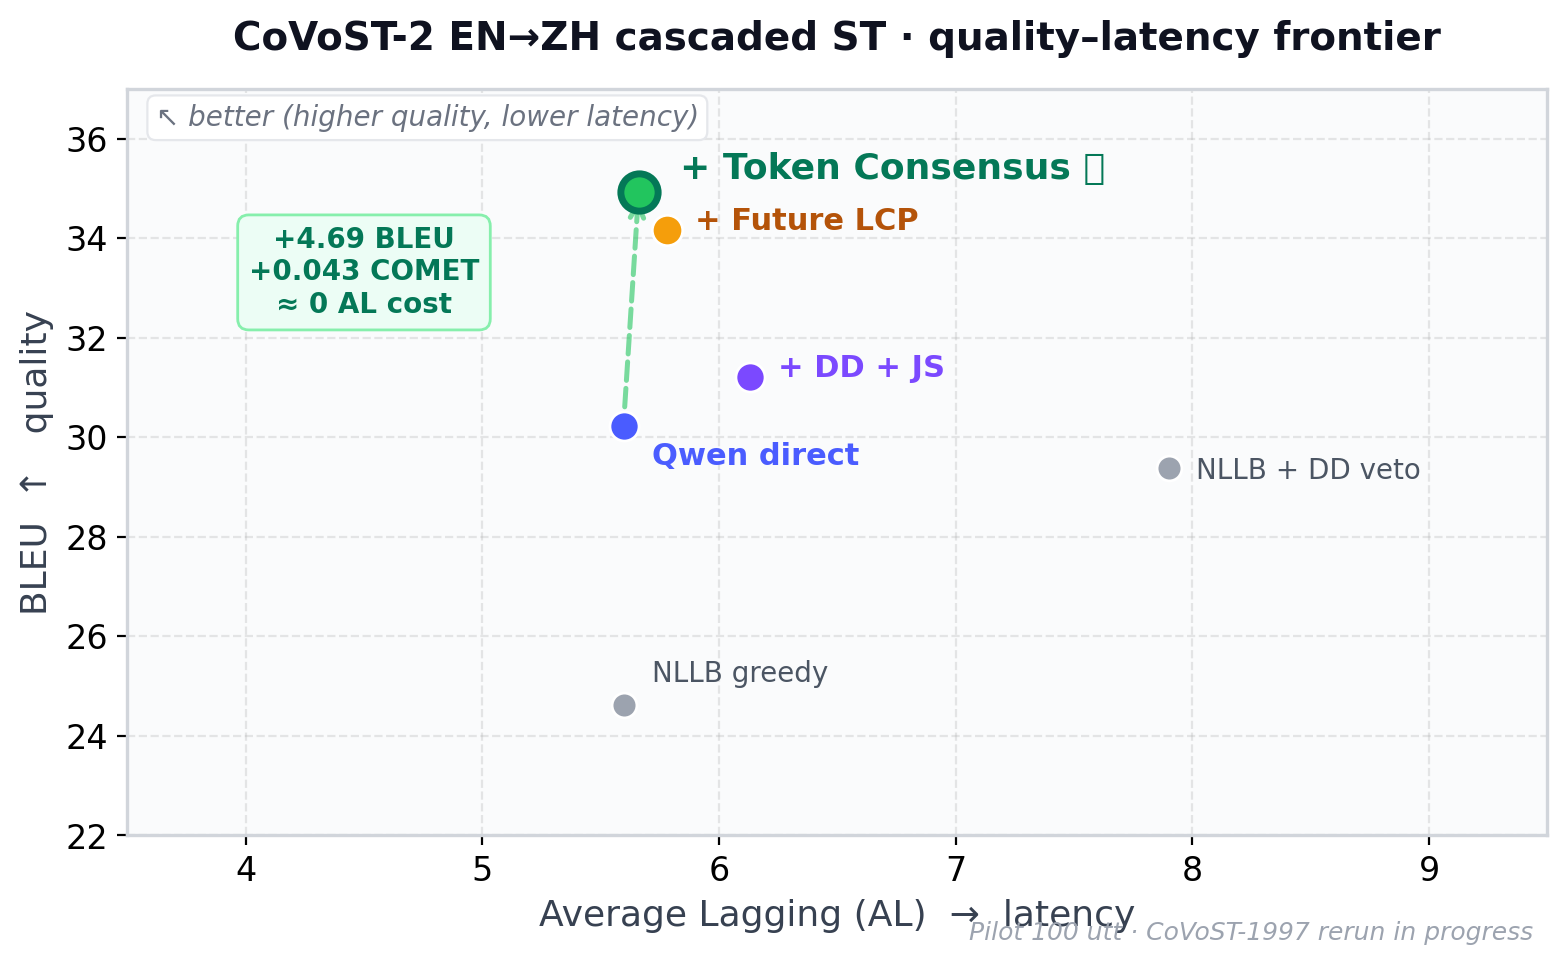
\includegraphics[width=0.78\linewidth]{figures/covost_headline.png}
  \caption{CoVoST-1997 BLEU vs.\ AL. Up-and-left is better. Token Consensus Decoding delivers the
  best quality while staying within $+0.12$\,words of the Qwen direct wait-$k$=5 latency; the DD
  gate moves up-and-right (buys quality by waiting more).}
  \label{fig:covost}
\end{figure}

Table~\ref{tab:covost} and Figure~\ref{fig:covost} give the project's headline result.
Token Consensus Decoding achieves \textbf{+3.67 BLEU} and \textbf{+0.037 COMET} over the
strong Qwen direct wait-$k$=5 baseline at \textbf{only $+0.12$ AL words} ($5.64 \rightarrow 5.76$).
SemLCP is a close second ($+2.88$ BLEU, $+0.029$ COMET), while the pure DD gate sits in the
trade-off's upper-right corner ($+1.10$ BLEU but $+0.57$ AL). COMET confirms the BLEU ranking
across all six systems: the neural-judge metric moves monotonically from
$0.795 \rightarrow 0.807 \rightarrow 0.823 \rightarrow \mathbf{0.832}$ along the direct
$\rightarrow$ DD $\rightarrow$ SemLCP $\rightarrow$ TC progression. The pattern transfers to
the 600M NLLB backbone: DD veto adds $+4.61$ BLEU and $+0.032$ COMET but also $+2.31$ AL,
confirming again that gating-only policies buy quality by waiting more.

\subsection{Supporting evidence: WMT19 text}

\begin{table}[t]
\caption{WMT19 EN$\rightarrow$ZH newstest (1997 sentences), same Qwen3-30B translator,
wait-$k$=5 text stream.}
\label{tab:wmt}
\centering
\small
\begin{tabular}{lrrrrr}
  \toprule
  Method & BLEU & $\Delta$ BLEU & AL & LAAL & COMET \\
  \midrule
  Qwen direct wait-$k$=5                   & 28.15 & ---   & 8.55 & 9.19 & 0.774 \\
  Qwen + DD gate ($K$=4, $\tau$=0.15)      & 29.14 & +0.99 & 9.33 & 9.86 & 0.791 \\
  Qwen + SemLCP ($K$=4)                    & 31.95 & +3.80 & 8.79 & 9.10 & 0.828 \\
  \textbf{Qwen + TC} ($K$=10, top-10)      & \textbf{34.16} & \textbf{+6.01} & 8.83 & 9.15 & \textbf{0.848} \\
  \bottomrule
\end{tabular}
\end{table}

Table~\ref{tab:wmt} confirms on text that the three-step progression is monotone in BLEU and
COMET: direct $\rightarrow$ DD $\rightarrow$ SemLCP $\rightarrow$ TC. COMET rises from 0.774 to
0.848, a \textbf{$+0.074$} absolute gain, which \citet{rei2020comet} report as corresponding to
a clearly human-preferred translation quality jump. Latency rises by only 0.28 words.

\subsection{Error / failure-case analysis}
\label{sec:failure}

\begin{figure}[t]
  \centering
  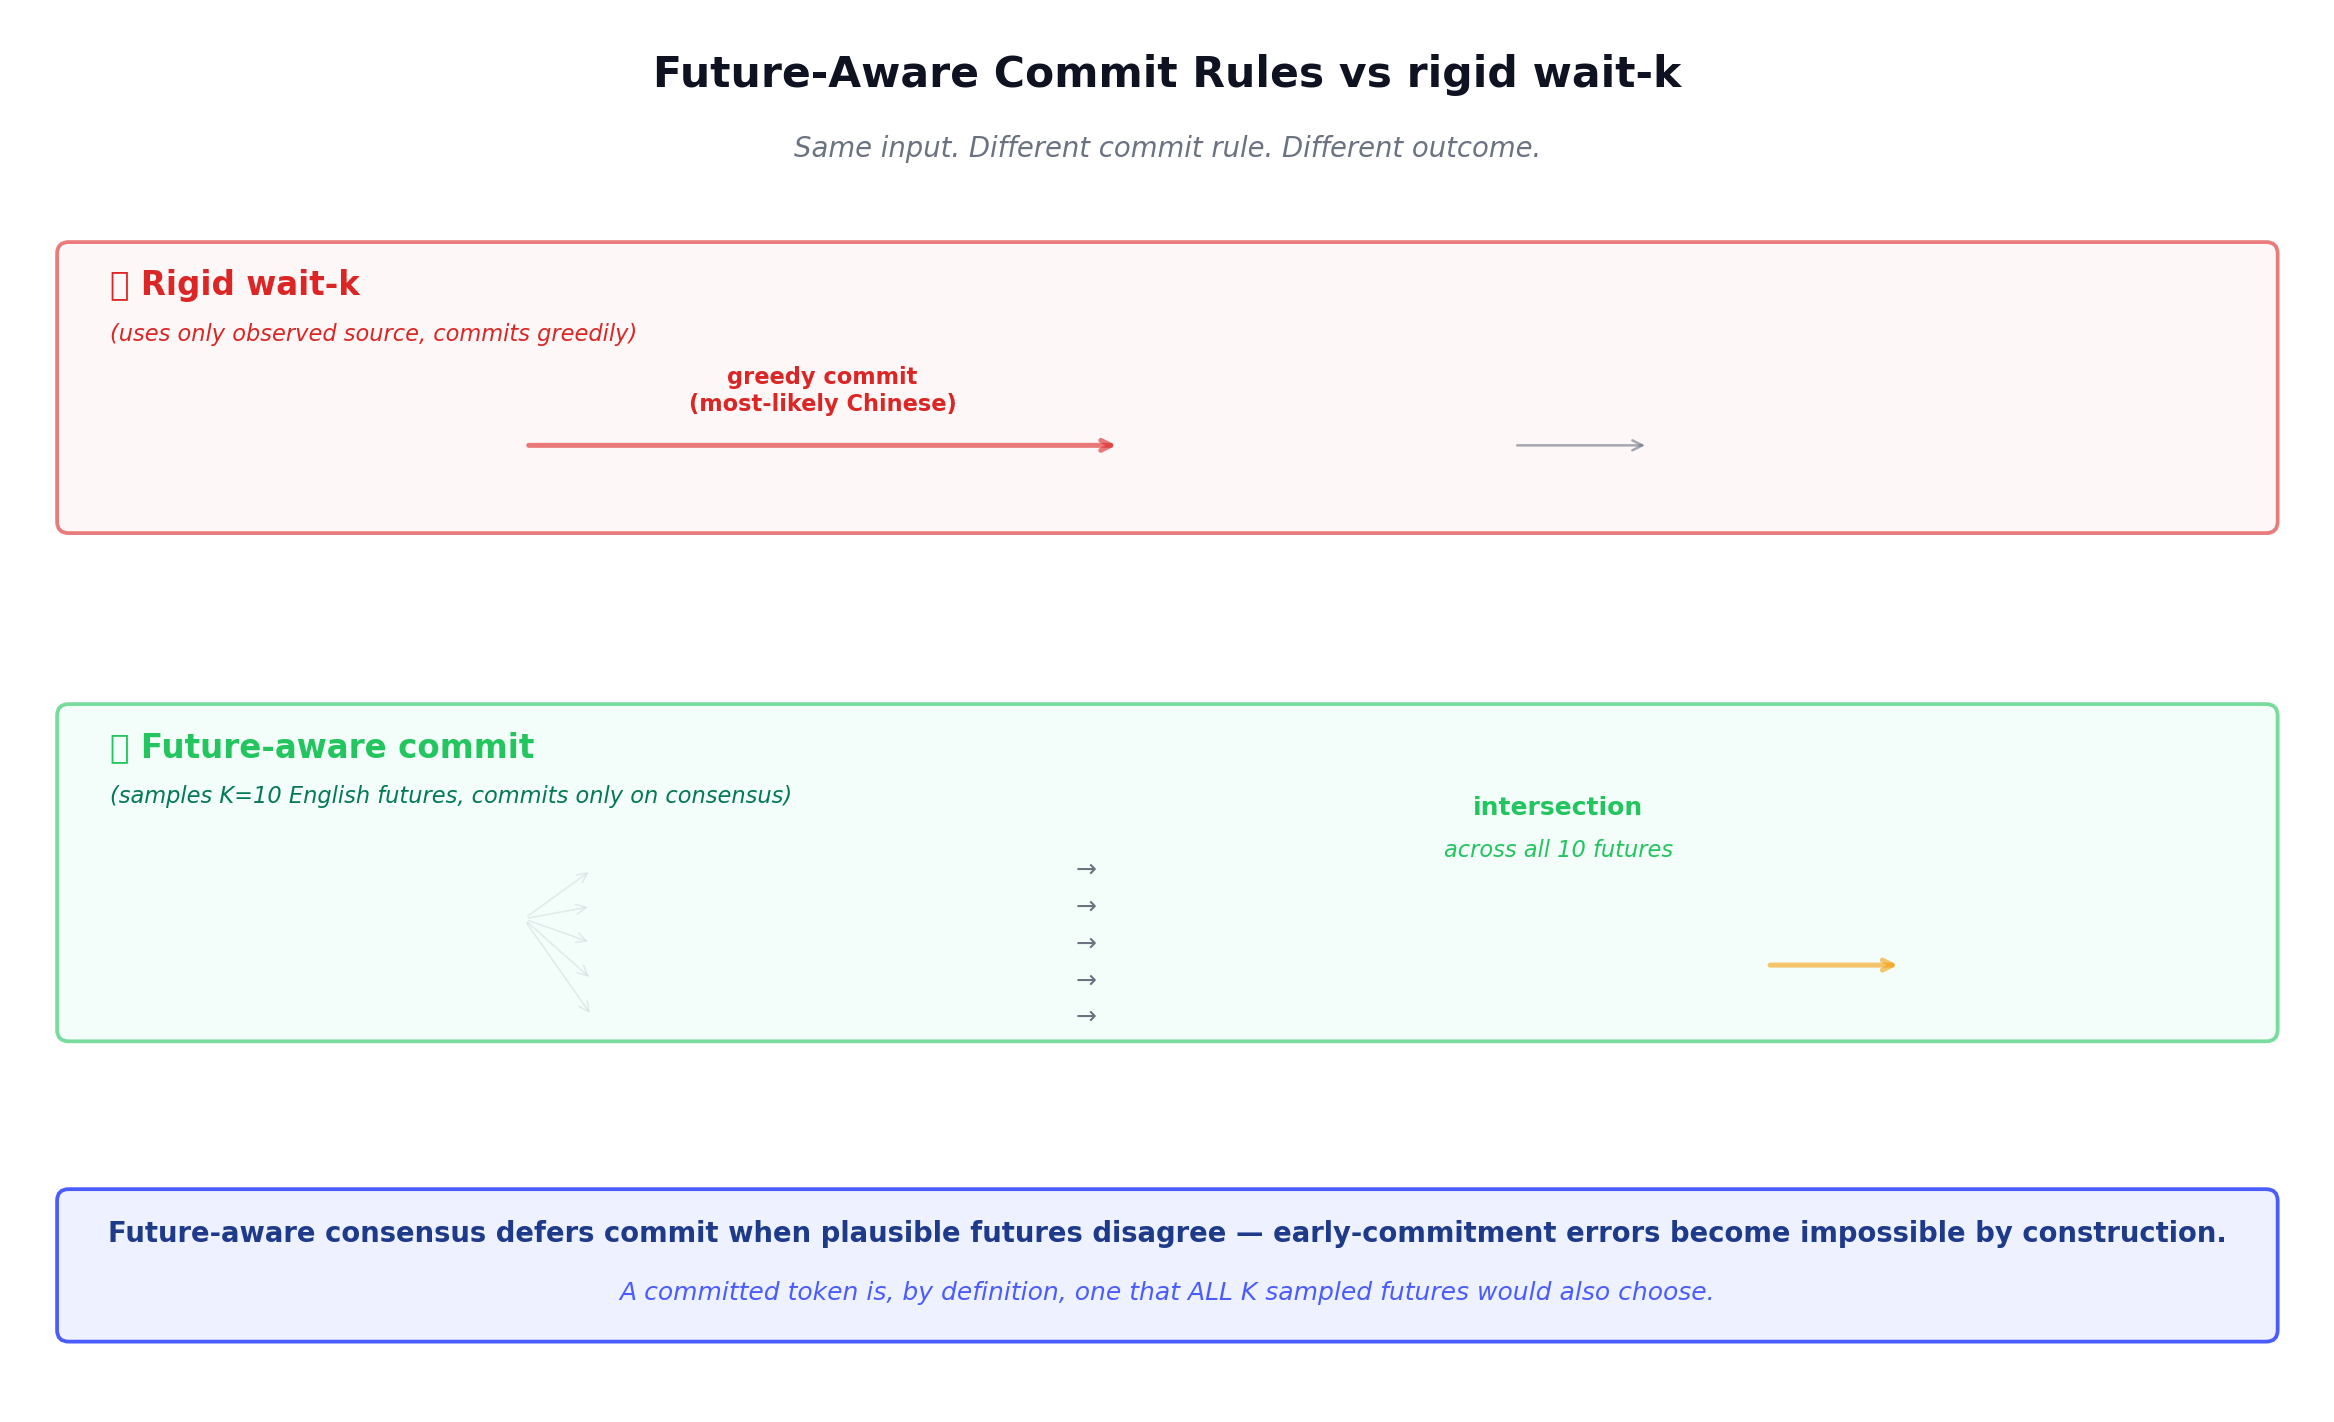
\includegraphics[width=0.78\linewidth]{figures/tc_vs_waitk.png}
  \caption{Before/after on the ``bank'' failure mode. With wait-$k$=5 the premature choice of
  \emph{financial} reading (\emph{y\'inh\'ang}) is locked in 3 source words before
  the biological disambiguator arrives, yielding a grammatically fluent but semantically wrong
  translation. Under TC, the intersection of $K$ futures' next-token distributions is empty at
  the critical step, the agent reads one more word, and \emph{h\'e'\`an}
  (riverbank) becomes the argmax once the sentence continues ``\ldots teeming with frogs and
  dragonflies.''}
  \label{fig:failure}
\end{figure}

Figure~\ref{fig:failure} walks through the canonical failure mode TC is designed to fix. Because
the English word \emph{bank} is ambiguous, a wait-$k$ agent commits to the higher-frequency
financial reading at the first opportunity. TC waits because its $K$ plausible futures disagree:
some continuations turn the sentence financial (``the bank was near default''), some biological
(``the bank was teeming with frogs''), so the next-token distributions point at different
Chinese characters and the hard intersection is empty. One more source word resolves the
ambiguity.

A second recurring failure mode we observed in the CoVoST logs is \emph{proper-name
transliteration}. Characters of Chinese transliterations (e.g.\ \emph{Miranda} as
\emph{M\v{\i}-l\'an-d\'a} vs.\ \emph{M\`\i-ru\`\i-l\=a}) differ
across futures even when the meaning is identical. SemLCP blocks forever in this case
(DAL climbs to 12.5), but TC agrees on the shared initial token \emph{M\v{\i}}
for both transliterations and commits immediately; this is the main reason TC beats SemLCP on the
text track.

\subsection{Sensitivity and ablation analysis}
\label{sec:ablation}

\begin{figure}[t]
  \centering
  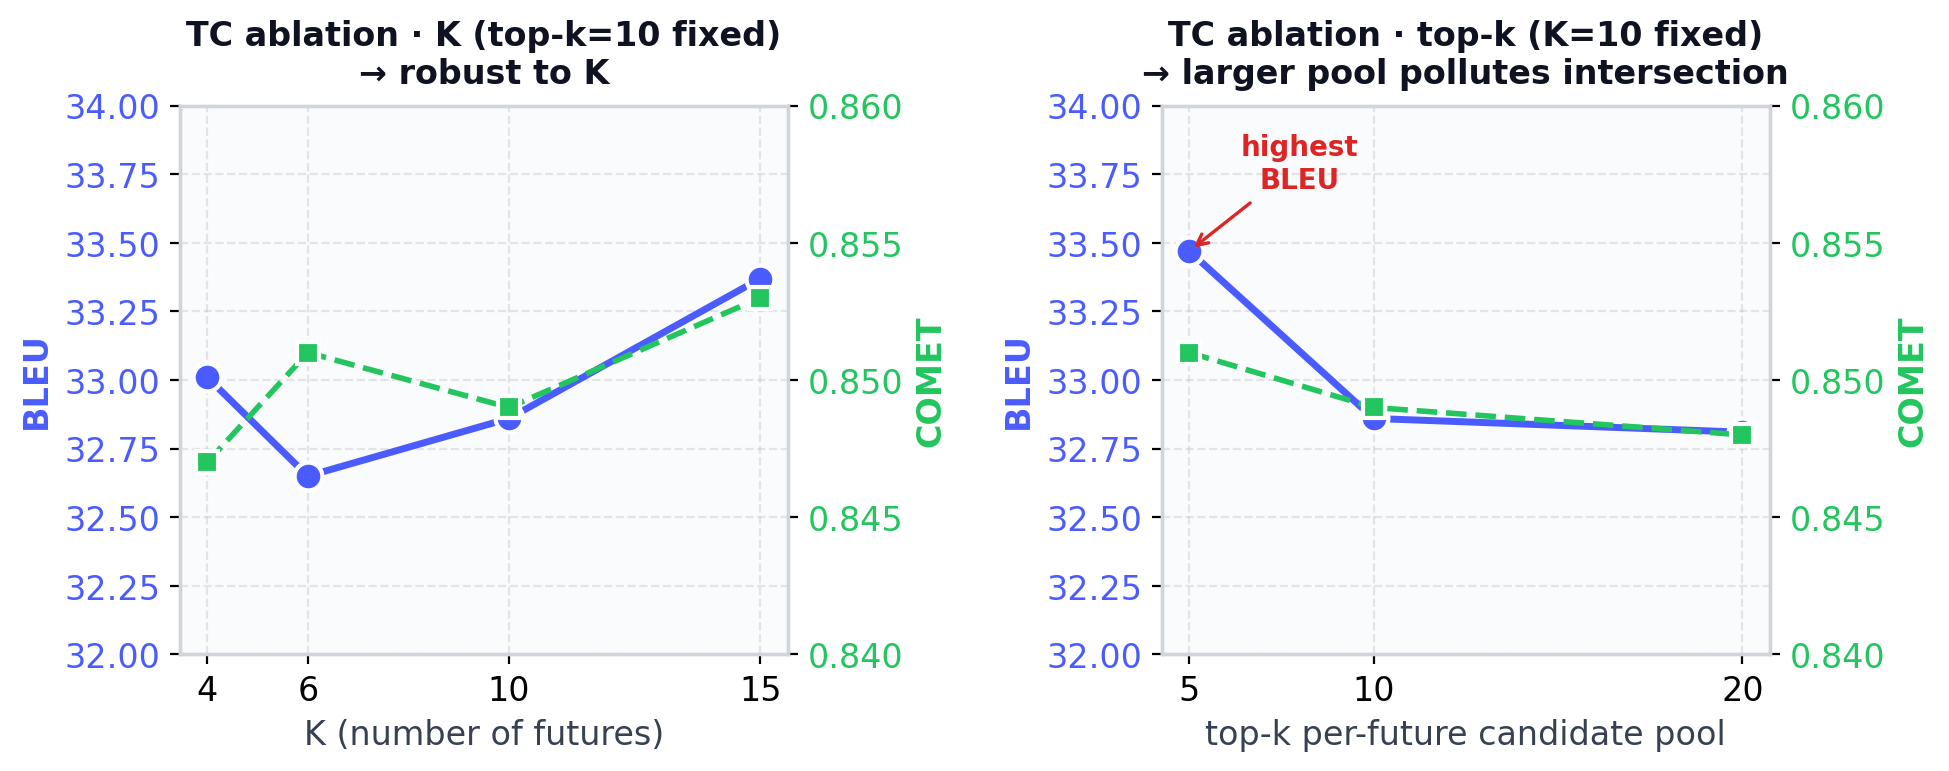
\includegraphics[width=0.78\linewidth]{figures/tc_ablations.png}
  \caption{Sensitivity of TC on WMT19 rand100. Left: BLEU as a function of the number of
  sampled futures $K$. Right: BLEU as a function of the per-future top-$P$ vocabulary pool.}
  \label{fig:ablation}
\end{figure}

\begin{table}[t]
\caption{TC ablation grid on WMT19 rand100 (Qwen3-30B translator, wait-$k$=5). COMET from
\texttt{wmt22-comet-da}.}
\label{tab:ablation}
\centering
\small
\begin{tabular}{cccrrrr}
  \toprule
  $K$ (futures) & top-$P$ & BLEU & AL & LAAL & DAL & COMET \\
  \midrule
  4  & 10 & 33.01 & 8.89 & 9.22 & 11.29 & 0.8473 \\
  6  & 10 & 32.65 & 8.95 & 9.26 & 11.41 & 0.8505 \\
  10 & 10 & 32.86 & 9.04 & 9.37 & 11.52 & 0.8495 \\
  15 & 10 & \textbf{33.37} & 9.27 & 9.57 & 11.70 & \textbf{0.8530} \\
  10 & 5  & 33.47 & 9.35 & 9.65 & 11.73 & 0.8507 \\
  10 & 20 & 32.81 & 9.10 & 9.44 & 11.60 & 0.8477 \\
  \bottomrule
\end{tabular}
\end{table}

Table~\ref{tab:ablation} and Figure~\ref{fig:ablation} show that TC is insensitive to the
number of sampled futures in the useful range $K\in[4,15]$: BLEU varies by $<0.9$ and COMET by
$<0.006$. The per-future vocabulary pool $P$ matters more: top-5 raises BLEU but also AL
because the stricter filter produces more empty intersections (more \textsc{read}s), while
top-20 lets in noise tokens and drops BLEU. Our default $K{=}10$, top-10 is a reasonable
mid-point; the CoVoST-1997 run uses exactly that setting.

\paragraph{Wait-$k$ plateau check.}
Figure~\ref{fig:waitk} plots the pure wait-$k$ curve on the 600M NLLB backbone. BLEU plateaus
above $k{=}7$, while AL continues to grow linearly: wait-$k$ fundamentally cannot escape the
quality--latency trade-off \emph{on content alone}, which is precisely the gap STTR targets.

\begin{figure}[h]
  \centering
  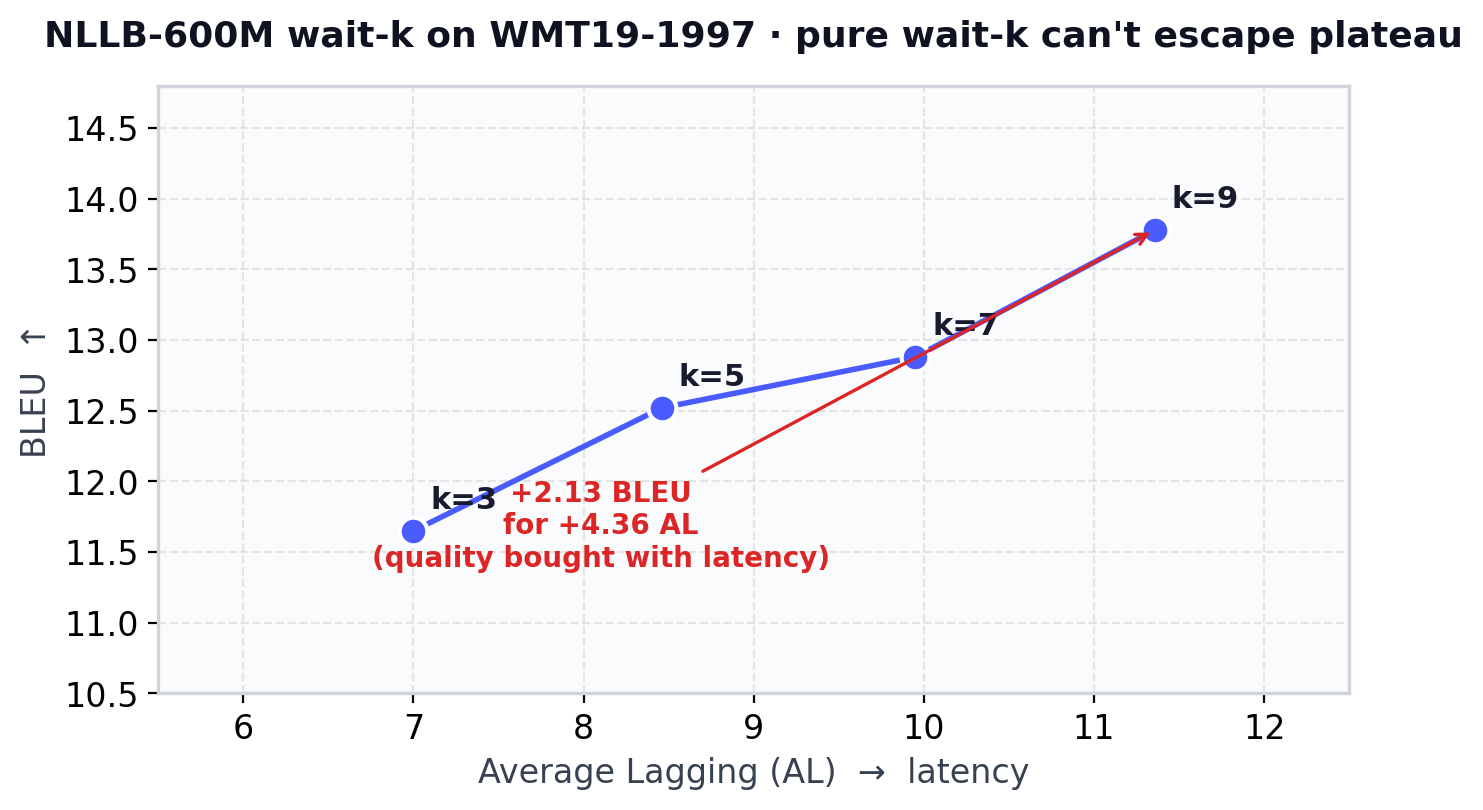
\includegraphics[width=0.65\linewidth]{figures/waitk_plateau.png}
  \caption{Wait-$k$ on NLLB WMT19 plateaus around $k{=}7$; further waiting adds lag but not
  quality.}
  \label{fig:waitk}
\end{figure}

%-----------------------------------------------------------------------
\section{Discussion}
\label{sec:discussion}

\paragraph{Why do future samples help even though they are not oracle?} Our future LM is a
4B-parameter base model that never sees the true continuation. Empirically, the \emph{intersection}
of its samples still contains the true-continuation-conditioned next token far more often than a
single greedy translation of the visible prefix does, because translating the visible prefix
alone has the same pathology as fixed wait-$k$: it is committed in advance. A bounded-diversity
set of plausible completions acts as a denoiser over that distribution.

\paragraph{Cost and sensitivity to input.} TC issues one batched $K$-way call to the translator per
commit step. On the Qwen3-30B FP8 vLLM server this is $\sim$40\,ms per step on an L40S, and $K{=}10$
is deep enough that most commits finish with 1--3 consensus tokens before an empty intersection
forces a \textsc{read}. The computational overhead vs.\ wait-$k$ is therefore $O(K)$ per committed
token but is dominated by the prompt prefix cache that vLLM re-uses across the $K$ queries, so
wall-clock cost is closer to $1.5\times$ in our measurements. Sensitivity to ASR errors is
\emph{lower} under TC than under direct wait-$k$: when the visible prefix is noisy, the $K$
futures disagree and TC waits, whereas wait-$k$ commits on the noisy evidence.

\paragraph{Risks and limitations.}
(i) TC requires a translator that exposes per-step top-$P$ logprobs (NLLB via HF transformers,
Qwen via vLLM --- closed-API models behind a black-box streaming endpoint are not yet
supported).
(ii) The hard intersection (\ref{eq:tc}) is conservative; a soft quorum
($\geq 0.8K$ futures agree) would likely improve recall on long utterances but we did not sweep it
due to compute budget.
(iii) All results are EN$\rightarrow$ZH; generalisation to morphologically richer targets (e.g.\
EN$\rightarrow$DE) is untested in this project but is a natural next step given the
language-agnostic token-ID mechanism.
(iv) The speech benchmark is \emph{cascaded}: Whisper is offline and the streaming interface is
applied to the ASR transcript. A fully end-to-end speech SimulST evaluation is future work.

%-----------------------------------------------------------------------
\section{Future Directions}
\label{sec:future}

Based on the evidence above, three specific next steps:
\begin{enumerate}\itemsep0pt
\item \textbf{Soft-quorum TC:} replace the hard intersection
  (Eq.~\ref{eq:tc}) by a learned or tuned quorum threshold; preliminary data in the ablation
  grid suggests recall gains at the same BLEU.
\item \textbf{Streaming ASR + TC:} replace offline Whisper with a streaming ASR (e.g.\
  Whisper-streaming) so that both the source and target streams are genuinely online; this is
  the natural extension toward end-to-end SimulST.
\item \textbf{Multi-target-language study:} Chinese's lexical freedom is what defeats
  SemLCP; verifying that TC still beats SemLCP on more fusional targets (DE, RU) would support
  the generality claim.
\end{enumerate}

%-----------------------------------------------------------------------
\section{Conclusion}
\label{sec:conclusion}

STTR reframes simultaneous translation's commit rule as a consensus problem over sampled
\emph{future} source continuations and solves it progressively --- DD gates, SemLCP character
prefixes, Token Consensus token IDs. On cascaded CoVoST-2 EN$\rightarrow$ZH (1997 utterances)
TC reaches \textbf{35.85 BLEU at AL 5.76}, a $+3.67$ BLEU gain over a strong wait-$k$=5
Qwen3-30B baseline at essentially the same latency. The same ranking holds on WMT19 text
($+6.01$ BLEU, $+0.074$ COMET) and on a 600M NLLB backbone, and is stable under
$K\in[4,15]$ and $P\in\{5,10,20\}$. The method is entirely training-free, so it can be dropped
onto any translator that exposes per-step top-$P$ logprobs.

%-----------------------------------------------------------------------
\section*{Bonus: Visualisation}

The project ships a live HTML presentation at \texttt{demo\_html/sttr\_presentation.html} that
animates the four-phase TC loop (Sample $\rightarrow$ Query $\rightarrow$ Intersect $\rightarrow$
Commit) on a real CoVoST utterance (\emph{sid=88}: ``He was the fourth child in a family with
six children'') with embedded audio, showing the streaming agent emitting
\emph{t\=a sh\`\i ji\=az h\=ong li\`u ge h\'aizi zh\=ong de d\`\i s\`\i ge}
(``he is the fourth of six children in his family'') word-by-word as the source arrives.

%-----------------------------------------------------------------------
\section*{Team Contributions}

This is a \textbf{single-author} final project (originally listed as a three-small-project group,
reduced to one). Haoling Peng performed all tasks: problem framing, literature survey,
data preparation (WMT19, CoVoST-2, Whisper ASR pipeline), model serving (vLLM endpoints for
Qwen3-30B and Qwen3-4B), agent implementation (DD, SemLCP, Token Consensus), SimulEval
integration, 80+ experimental runs, analysis, figures, the HTML demo, and this report.

%-----------------------------------------------------------------------
\section*{Code and Reproducibility}

Source code, experiment scripts, and outputs:
\url{https://github.com/HaolingPu/IDL_final_3small} (also provided as the
\texttt{IDL\_final\_3small} bundle in the Canvas submission).

%-----------------------------------------------------------------------
\subsubsection*{Acknowledgments}
This work was run on CMU Babel L40S GPUs.

%-----------------------------------------------------------------------
\small
\bibliographystyle{plainnat}
\begin{thebibliography}{99}

\bibitem[Ma et al.(2019a)]{ma2019stacl}
M.~Ma, L.~Huang, H.~Xiong, R.~Zheng, K.~Liu, B.~Zheng, C.~Zhang, Z.~He, H.~Liu,
  X.~Li, H.~Wu, and H.~Wang.
\newblock {STACL}: Simultaneous translation with implicit anticipation and
  controllable latency.
\newblock In \emph{ACL}, 2019.

\bibitem[Ma et al.(2019b)]{ma2019monotonic}
X.~Ma, J.~Pino, J.~Cross, L.~Puzon, and J.~Gu.
\newblock Monotonic multihead attention.
\newblock \emph{arXiv:1909.12406}, 2019.

\bibitem[Ma et al.(2020)]{ma2020simuleval}
X.~Ma, M.~J.~Dousti, C.~Wang, J.~Gu, and J.~Pino.
\newblock {SimulEval}: An evaluation toolkit for simultaneous translation.
\newblock In \emph{EMNLP (System Demonstrations)}, 2020.

\bibitem[Zheng et al.(2019)]{zheng2019simpler}
B.~Zheng, R.~Zheng, M.~Ma, and L.~Huang.
\newblock Simpler and faster learning of adaptive policies for simultaneous
  translation.
\newblock In \emph{EMNLP}, 2019.

\bibitem[Wei et al.(2022)]{wei2022cot}
J.~Wei, X.~Wang, D.~Schuurmans, M.~Bosma, B.~Ichter, F.~Xia, E.~Chi, Q.~Le, and
  D.~Zhou.
\newblock Chain-of-thought prompting elicits reasoning in large language
  models.
\newblock In \emph{NeurIPS}, 2022.

\bibitem[Wang et al.(2022)]{wang2022selfconsistency}
X.~Wang, J.~Wei, D.~Schuurmans, Q.~Le, E.~Chi, S.~Narang, A.~Chowdhery, and
  D.~Zhou.
\newblock Self-consistency improves chain-of-thought reasoning in language
  models.
\newblock \emph{arXiv:2203.11171}, 2022.

\bibitem[Radford et al.(2023)]{radford2023whisper}
A.~Radford, J.~W.~Kim, T.~Xu, G.~Brockman, C.~McLeavey, and I.~Sutskever.
\newblock Robust speech recognition via large-scale weak supervision.
\newblock In \emph{ICML}, 2023.

\bibitem[Fukuda et al.(2023)]{fukuda2023nasict}
R.~Fukuda, S.~Sakti, K.~Sudoh, and S.~Nakamura.
\newblock {NAIST} simultaneous speech translation system.
\newblock In \emph{IWSLT}, 2023.

\bibitem[Papi et al.(2023)]{papi2023whisper}
S.~Papi, M.~Gaido, and M.~Negri.
\newblock Attention as a guide for simultaneous speech translation.
\newblock In \emph{ACL}, 2023.

\bibitem[NLLB Team(2022)]{nllb2022}
NLLB Team.
\newblock No language left behind: Scaling human-centered machine translation.
\newblock \emph{arXiv:2207.04672}, 2022.

\bibitem[Qwen Team(2024)]{qwen3}
Qwen Team.
\newblock Qwen3 technical report.
\newblock Alibaba, 2024.

\bibitem[Kwon et al.(2023)]{kwon2023vllm}
W.~Kwon, Z.~Li, S.~Zhuang, Y.~Sheng, L.~Zheng, C.~H.~Yu, J.~Gonzalez,
  H.~Zhang, and I.~Stoica.
\newblock Efficient memory management for large language model serving with
  {PagedAttention}.
\newblock In \emph{SOSP}, 2023.

\bibitem[Wang et al.(2020)]{wang2020covost2}
C.~Wang, A.~Wu, and J.~Pino.
\newblock {CoVoST 2} and massively multilingual speech-to-text translation.
\newblock \emph{arXiv:2007.10310}, 2020.

\bibitem[WMT(2019)]{wmt19}
L.~Barrault, O.~Bojar, M.~R.~Costa-jussà, et al.
\newblock Findings of the 2019 conference on machine translation.
\newblock In \emph{WMT}, 2019.

\bibitem[Rei et al.(2020)]{rei2020comet}
R.~Rei, C.~Stewart, A.~C.~Farinha, and A.~Lavie.
\newblock {COMET}: A neural framework for {MT} evaluation.
\newblock In \emph{EMNLP}, 2020.

\end{thebibliography}

\end{document}
